\graphicspath{{../../S24_la_Proportionnalite/Images/}}

\themeO
\chapter{La proportionnalité}
\label{S24}

\programme%
   {\item Coefficient de proportionnalité.}
   {\item Reconnaître une situation de proportionnalité ou de non-proportionnalité.
    \item Résoudre des problèmes utilisant la proportionnalité (pourcentages, échelles, agrandissement réduction).}

\vfill

\begin{debat}{Débat : ces affreux pourcentages !}
   La notion de {\bf pourcentage} est très importante dans la vie courante mais c'est un concept relativement mal compris ou mal utilisé, et on trouve régulièrement des erreurs dans les médias. Ces deux vidéos montrent des exemples de pourcentages erronés dans des journaux d'information.
   \tcblower
      \fontsize{70}{80}\selectfont \%
\end{debat}

\hfill {\gray Vidéos : \href{https://www.youtube.com/watch?v=gLbsxj8mv-U}{\bf Facture d'électricité} et \href{https://www.youtube.com/watch?v=gXcwdDYSMeM&t=118s}{\bf Appliquer un pourcentage}, chaîne Youtube {\it Rapémathiques} d'A'Rieka.}


%%% Approche %%%
\begin{Maquette}[Cours]{Theme={Activité d'approche},Couleur={SteelBlue}}

   \AAtitre{Le puzzle de Brousseau}

      {\it Objectifs : mettre en \oe uvre un ou des moyens pour résoudre un problème d'agrandissement ; reproduire une figure géométrique en respectant des mesures ; rendre compte d'un travail en groupe.}

      \begin{AActivite}

         \AApartie{Présentation du puzzle}
            Ci-dessous se trouve un puzzle carré composé de cinq pièces A, B, C, D et E dont les mesures sont indiquées sur la figure. 
            \begin{center}
               \begin{pspicture}(-1,-1)(12,12)
                  \psframe(0,0)(11,11)
                  \psframe(4,0)(3.7,0.3)
                  \psframe(11,9)(10.7,8.7)
                  \psline(4,0)(4,9)(11,2)
                  \psline(6,11)(0,5)
                  \psline(11,9)(4,9)
                  \rput(2,9){\bf\large A}
                  \rput(8.5,10){\bf\large B}
                  \rput(8.5,7){\bf\large C}
                  \rput(2,4){\bf\large D}
                  \rput(7,3){\bf\large E}
                  \rput{90}(11.5,5.5){\Lg{7}}
                  \rput{90}(11.5,1){\Lg{2}}
                  \rput(8.5,11.5){\Lg{5}}
                  \rput(3,11.5){\Lg{6}}
                  \rput{90}(-0.5,8){\Lg{6}}
                  \rput{90}(-0.5,2.5){\Lg{5}}
                  \rput(2,-0.5){\Lg{4}}
                  \rput(7.5,-0.5){\Lg{7}}
                  \rput{90}(3.5,4.5){\Lg{9}}
                  \rput{90}(11.5,10){\Lg{2}}
                  \rput(8,8.5){\Lg{7}}
               \end{pspicture}
            \end{center}

         \AApartie{Travail demandé}
            Par groupes, vous allez devoir refaire le même puzzle mais en plus grand : il faudra s'accorder sur la procédure à adopter pour agrandir les éléments du puzzle, se répartir la construction des pièces en faisant les calculs individuellement puis assembler les morceaux pour reconstituer le puzzle agrandi. \par
            Le compte-rendu de vos recherches sera présenté sous la forme d’une affiche par groupe.
            \begin{center}
               {\bf C'est parti\dots{} le segment de \Lg{4} devra mesurer \Lg{5} sur votre puzzle agrandi.}
            \end{center}

      \end{AActivite}

\end{Maquette}


%%%Trace écrite %%%
\begin{Maquette}[Cours]{Theme={Trace écrite},Couleur={0.4[SteelBlue,Black]}}

   %%%1
   \section{Procédures de proportionnalité (rappels)}

      \begin{center}
         \begin{pspicture}(-0.5,3.9)(15.5,8.6)
            \psellipse[fillstyle=solid,fillcolor=Crimson!50](8,6.25)(2.7,1)
            \rput(8,6.25){\parbox{4.5cm}{\centering \bf Si 4 stylos coûtent \Prix{10} \par combien coûtent 12 stylos ?}}
            \psframe*[fillstyle=solid,linecolor=DodgerBlue!80](0.5,7)(7,8.6)
            \rput(3.75,7.8){\parbox{6.5cm}{\centering {\bf Linéarité additive} \par 12 stylos = 4 stylos + 4 stylos + 4 stylos \par coûtent \Prix{10} +\Prix{10} + \Prix{10} = \Prix{30}}}
            \psframe*[fillstyle=solid,linecolor=DodgerBlue!60](9,7)(13.5,8.6)
            \rput(11.25,7.8){\parbox{4.5cm}{\centering {\bf Linéarité multiplicative} \par 12 stylos = 3$\times$4 stylos \par coûtent $3\times\Prix{10} =\Prix{30}$}}
            \psframe*[fillstyle=solid,linecolor=DodgerBlue!40](-0.5,3.9)(7.5,5.5)
            \rput(3.5,4.7){\parbox{8cm}{\centering {\bf Passage par l'unité} \par 1 stylo coûte 4 fois moins cher : $\Prix{10}\div4 =\Prix{2,5}$ \par 12 stylos coûtent 12 fois plus cher : $12\times\Prix{2,5} =\Prix{30}$}}
            \psframe*[fillstyle=solid,linecolor=DodgerBlue!20](8.5,3.9)(15.5,5.5)
            \rput(12,4.7){\parbox{7cm}{\centering {\bf Coefficient de proportionnalité} \par coefficient de proportionnalité : $10\div4 =2,5$ \par 12 stylos coûtent \Prix{30} : $12\times\fbox{2,5} =30$}}
         \end{pspicture}
      \end{center}


%%%2
\section{Pourcentages}

   \begin{definition*}{}
      Le {\bf pourcentage} est le nombre qui aurait été proportionnellement obtenu si la quantité avait été de 100.
   \end{definition*}

   \begin{propriete*}{}
      Appliquer un taux de $t\,\%$ à une quantité revient à calculer $\dfrac{t}{100}$ de cette quantité.
   \end{propriete*}

   \begin{exemple*}{}
      Une promotion sur un jus de fruits indique que la contenance est de \Capa{1} + 20\,\%. \par
      Calcul de l'augmentation : $\dfrac{20}{100}\times\Capa{1} =\Capa{0,2}$. \par
      Calcul de la nouvelle contenance : $\Capa{1}+\Capa{0,2} =\Capa{1,2}$.
   \end{exemple*}

   Certains taux sont des pourcentages de référence :
   \begin{center}
      {\hautab{1.5}
      \begin{tabular}{|*4{C{2}|}p{4.3cm}}
         \rowcolor{lightgray} pourcentage & opération & facteur & vocabulaire & exemple avec un prix de \Prix{80} \\
         \cline{1-4}
         50\,\% & $\div2$ & $\frac12$ & la moitié & \Prix{40} \\
         25\,\% & $\div4$ & $\frac14$ & le quart & \Prix{20} \\
         20\,\% & $\div5$ & $\frac15$ & le vingtième & \Prix{16} \\
         10\,\% & $\div10$ & $\frac{1}{10}$ & le dixième & \Prix{8} \\
         1\,\% & $\div100$ & $\frac{1}{100}$ & le centième & \Prix{0,8} \\
         \cline{1-4}
      \end{tabular}}
   \end{center}


%%%3
\section{Échelles}

   \begin{definition*}{}
      L'\textbf{échelle} d'une carte est le coefficient de proportionnalité entre la mesure réelle et sa mesure sur la carte, ces deux mesures étant exprimées dans la même unité.
   \end{definition*}

   \begin{exemple*}{}
      Une carte au 1/\num{2000} signifie que \Lg{1} sur la carte représente \Lg{2000} en réalité, soit \Lg[m]{20}. On note aussi 1:\num{2000}.
      \Propor[GrandeurA={Distance sur la carte en cm},GrandeurB={Distance dans la réalité en m}]{1/20,2/40,10/200}
      \FlechesPD{1}{2}{$\times20$} \vspace*{-6mm}
   \end{exemple*}

\end{Maquette}


%%% Exercices %%%
\begin{Maquette}[Fiche,CorrigeFin,Colonnes=2]{}

   \begin{multicols}{2}

      \begin{exercice} %1
         Ces situations sont-elles proportionnelles ? \par
         Justifier par un contre-exemple ou une preuve.
         \begin{enumerate}
            \item Taille en mètre en fonction de l'âge ?
            \item Périmètre du carré en fonction de son côté ?
            \item Aire du carré en fonction de son côté ?
            \item Distance parcourue à vélo à vitesse constante en fonction du temps.
         \end{enumerate}
      \end{exercice}
      
      \begin{Solution}
         \begin{enumerate}
            \item \cor{Non}. Par exemple, si un enfant mesure \Lg{75} à 1 an, il ne mesurera pas $\Lg{750} =\Lg[m]{7,5}$ à 10 ans.
            \item \cor{Oui}. $\mathcal{P} =4\times c$, 4 étant une constante.
            \item \cor{Non}. Par exemple, un carré de côté \Lg{1} a une aire de \Aire{1} et un carré de côté \Lg{2} a une aire de \Aire{4}.
            \item \cor{Oui}. $d =v\times t$, la vitesse étant constante.
         \end{enumerate}
      \end{Solution}
      
      
      \begin{exercice}[SLF] %2
         Compléter les tableaux de proportionnalité suivants du prix d'un objet selon la quantité. \par \vskip-5mm
         \quad \Propor[GrandeurA=Objets,GrandeurB=Prix (\Prix{}),Math,Stretch=1.5,Largeur=7mm]{1/,12/,8/24,/75}
         \FlechesPD{1}{2}{$\times\dots$}
         \FlechesPG{2}{1}{$\times\dots$} \par \vskip-1cm
         \quad \Propor[GrandeurA=Objets,GrandeurB=Prix (\Prix{}),Math,Stretch=1.5,Largeur=7mm]{/3,/10,/26,60/}
         \FlechesPD{1}{2}{$\div5$}
         \FlechesPG{2}{1}{$\times\dots$} \par \vspace*{-5mm}
      \end{exercice}
      
      \begin{Solution}
         \Propor[GrandeurA=Objets,GrandeurB=Prix,Math,Stretch=1.5,Largeur=7mm,CouleurTab=Grey]{1/\textcolor{RoyalBlue}{3},12/\textcolor{RoyalBlue}{36},8/24,\textcolor{RoyalBlue}{25}/75}
         \quad \FlechesPD{1}{2}{\cor{$\times3$}}
         \FlechesPG{2}{1}{\cor{$\times\frac13$}} \par \vskip-1cm
         \quad \Propor[GrandeurA=Objets,GrandeurB=Prix,Math,Stretch=1.5,Largeur=7mm,CouleurTab=Grey]{\textcolor{RoyalBlue}{15}/3,\textcolor{RoyalBlue}{50}/10,\textcolor{RoyalBlue}{130}/26,60/\textcolor{RoyalBlue}{12}}
         \FlechesPD{1}{2}{$\div5$}
         \FlechesPG{2}{1}{\cor{$\times5$}} \par \vspace{-5mm}
      \end{Solution}
      
      
      \begin{exercice} %3
         Léon a pesé ses beignets et a trouvé que deux beignets pèsent \Masse{300} et trois beignets pèsent \Masse{450}.
         \begin{enumerate}
            \item Combien pèsent cinq beignets ?
            \item Combien pèsent six beignets ?
            \item Combien pèsent quatorze beignets ?
         \end{enumerate}
      \end{exercice}
      
      \begin{Solution}
         \begin{enumerate}
            \item 5 beignets $=$ 2 beignets $+$ 3 beignets. \par
               Or, $\Masse{300}+\Masse{450} =\Masse{750}$. \par
               Donc, \cor{5 beignets pèsent \Masse{750}}.
            \item 6 beignets $=2\times3$ beignets.
               Or, $2\times\Masse{450} = \Masse{900}$. \par
               Donc, \cor{6 beignets pèsent \Masse{900}}.
            \item 14 beignets $=7\times2$ beignets. \par
               Or, $7\times\Masse{300} =\Masse{2100}$. \par
               Donc, \cor{14 beignets pèsent \Masse{2100}}.
         \end{enumerate}
      \end{Solution}
      
      
      \begin{exercice} %4
         \begin{enumerate}
            \item Un cycliste roule à la vitesse moyenne de \Vitesse{24}. Combien de temps va-t-il mettre pour effectuer son circuit de \Lg[km]{36} ?
            \item Un cycliste roule pendant \Temps{;;;2} et parcourt \Lg[km]{34}. Quelle a été sa vitesse moyenne ?
         \end{enumerate}
      \end{exercice}
      
      \begin{Solution}
         \begin{enumerate}
            \item Le cycliste parcourt \Lg[km]{24} en \Temps{;;;1}, soit \Lg[km]{12} en \Temps{;;;;30} (2 fois moins), et donc \cor{\Lg[km]{36} en \Temps{;;;1;30}} (3 fois plus).
            \item Le cycliste parcourt \Lg[km]{34} en \Temps{;;;2}, donc \Lg[km]{17} en \Temps{;;;1}. \par
               \cor{Sa vitesse moyenne est donc de \Vitesse{17}}.
         \end{enumerate}
      \end{Solution}


      \begin{exercice}[Dur] %5
         Un robinet qui fuit laisse échapper de façon continue trois litres d’eau en deux heures.
         \begin{enumerate}
            \item Quelle quantité d’eau se sera écoulée au bout d’une demi-journée ?
            \item Quel temps s’est écoulé pour laisser s’échapper \Capa{51} ?
            \item L’eau est facturée \Prix{0,0031} le litre. \\
               Quel sera le montant de la facture au bout d’un an ?
         \end{enumerate}
      \end{exercice}
      
      \begin{Solution}
         \begin{enumerate}
            \item Une demi-journée dure \Temps{;;;12}, c'est-à-dire $6\times\Temps{;;;2}$. \\
               La quantité d'eau écoulée sera de $6\times\Capa{3} =\cor{\Capa{18}}$.
            \item $\Capa{51} =17\times\Capa{3}$. \\
               Il s'est donc écoulé $17\times\Temps{;;;2} =\cor{\Temps{;;;34}}$.
            \item Un an, c'est 365 jours, soit 730 demi-journées. \\
               Il s'écoulera donc $730\times\Capa{18} =\Capa{13140}$ en un an. \\
               À 0,0031\euro{} le litre, cela fait $13140\times0,0031\text{\euro} \approx\cor{\Prix{41}}$.
         \end{enumerate}
      \end{Solution}
      
      
      \begin{exercice} %6
         Au collège de Yuhithan, le foyer prend en charge 25\,\% du prix des voyages scolaires alors que dans celui d'Emmanuel, le foyer donne \Prix{54} pour un voyage de \Prix{180} et l'aide est proportionnelle au coût du voyage.
         \begin{enumerate}
            \item Si Yuhithan participe à un voyage qui coûte \Prix{230}, quel montant est pris en charge par son foyer ?
            \item En proportion, dans quel collège le foyer participe-t-il le plus au financement des voyages ?
         \end{enumerate}
      \end{exercice}
      
      \begin{Solution}
         \begin{enumerate}
            \item $\dfrac{25}{100}\times\Prix{230} =\Prix{57,5}$. \par \smallskip
               Sur \Prix{230}, \cor{\Prix{57,5} sont pris en charge par le foyer}.
            \item Au collège de Yuhithan, le pourcentage pris en charge est de $\dfrac{\Prix{54}}{\Prix{180}}\times100 =30\%$. \par C'est donc au \cor{collège de Ginan que la proportion prise en charge par le foyer est la plus élevée}.
         \end{enumerate}
      \end{Solution}
      
      
      \begin{exercice} %7
         Selene fait pour ses amis deux verres contenant des boissons au sirop.
            \begin{enumerate}
               \item Le premier verre a une contenance de \Capa[cL]{20} et il y a 3,5\,\% de sirop. Combien cela fait-il de sirop ?
               \item Le deuxième verre contient \Capa[cL]{10} de boisson dont 5\,\% de sirop. Combien cela fait-il de sirop ?
               \item Sachant qu'au départ, il y avait \Capa[mL]{15} de sirop, combien lui reste-t-il de sirop après ces deux verres ?
            \end{enumerate}
      \end{exercice}
         
      \begin{Solution}
         \begin{enumerate}
            \item 1\up{er} verre : $\dfrac{3,5}{100}\times\Capa[cL]{20} =\Capa[cL]{0,7}$. \par
               \cor{Le premier verre contient \Capa[cL]{0,7} de sirop}.
            \item 2\up{e} verre : $\dfrac{5}{100}\times\Capa[cL]{10} =\Capa[cL]{0,5}$.
               \cor{Le deuxième verre contient \Capa[cL]{0,7} de sirop}.
            \item Dans les verres, il y a $\Capa[cL]{0,7}+\Capa[cL]{0,5} =\Capa[cL]{1,2}$ de sirop. \par
               Au départ, Selene avait $\Capa[mL]{15} = \Capa[cL]{1,5}$, \cor{il lui restera donc \Capa[cL]{0,3} de sirop}.
         \end{enumerate}
      \end{Solution}
      
      
      \begin{exercice} %8
         Reproduire sur le cahier la cocotte à l'échelle 1:2 puis à l'échelle 2:1.
         \begin{center}
            \psset{unit=0.5}
            \begin{pspicture}(8,8)
               \psgrid[subgriddiv=1,linestyle=solid,gridlabels=0,gridcolor=Grey](0,0)(8,8)
               \psset{linewidth=0.5mm}
               \pspolygon(1,1)(4,1)(5.5,2.5)(7,1)(7,4)(5.5,5.5)(7,7)(4,7)(4,4)
            \end{pspicture}
         \end{center} 
      \end{exercice}
      
      \begin{Solution}
         Échelle $1:2$. \cor{On divise les mesures par 2}. \par
         {\psset{unit=0.5}
            \begin{pspicture}(-5,-0.5)(5,5.5)
               \psgrid[subgriddiv=1,linestyle=solid,gridlabels=0,gridcolor=Grey](0,0)(5,5)
            \psset{unit=0.5}
               \psset{linewidth=0.5mm}
               \pspolygon(2,2)(5,2)(6.5,3.5)(8,2)(8,5)(6.5,6.5)(8,8)(5,8)(5,5)         
            \end{pspicture}} \\
         Échelle $2:1$. \cor{On multiplie les mesures par 2}. \par
            {\psset{unit=0.5}
               \begin{pspicture}(0,-0.5)(13,14.5)
               \psgrid[subgriddiv=1,linestyle=solid,gridlabels=0,gridcolor=Grey](0,0)(14,14)
               \psset{linewidth=0.5mm}
               \pspolygon(1,1)(7,1)(10,4)(13,1)(13,7)(10,10)(13,13)(7,13)(7,7)
            \end{pspicture}}
      \end{Solution}
      
      
      \begin{exercice}[Dur] %9
         Trois poules pondent dix \oe ufs en deux heures.
         \begin{enumerate}
            \item Combien de poules faudrait-il pour pondre cinq \oe ufs en vingt minutes ?
            \item Combien de temps mettraient neuf poules pour pondre vingt \oe ufs ?
         \end{enumerate}
      \end{exercice}
      
      \begin{Solution}
         \begin{enumerate}
            \item 3 poules pondent 5 \oe ufs en $\Temps{;;;1} =\Temps{;;;;60}$ ; \par
               donc, \cor{9 poules pondent 5 \oe ufs en \Temps{;;;;20}} (il faut 3 fois plus de poules pour 3 fois moins de temps). \par
            \item 9 poules pondent 5 \oe ufs en \Temps{;;;;20} ; \par
               donc, \cor{9 poules pondent 20 \oe ufs en \Temps{;;;;80}} (il y a 4 fois plus d'\oe ufs, il faut 4 fois plus de temps).
         \end{enumerate}
      \end{Solution}

   \end{multicols}

\end{Maquette}


%%% Récré %%%
\begin{Maquette}[Cours]{Theme={Activité récréative},Couleur={IndianRed}}
    
   \ARtitre{Empreinte carbone}
      
      \ARpartie{Une infographie}
         Voici un extrait d’un document paru dans le quotidien {\it Le Monde} (infographie d’Hélène Pasquier), élaboré à partir de l’Ademe, et intitulé \og Rapport des inégalités du monde 2022 \fg, d’après le ministère de la transition écologique et le Haut conseil pour le climat. \par \smallskip 
         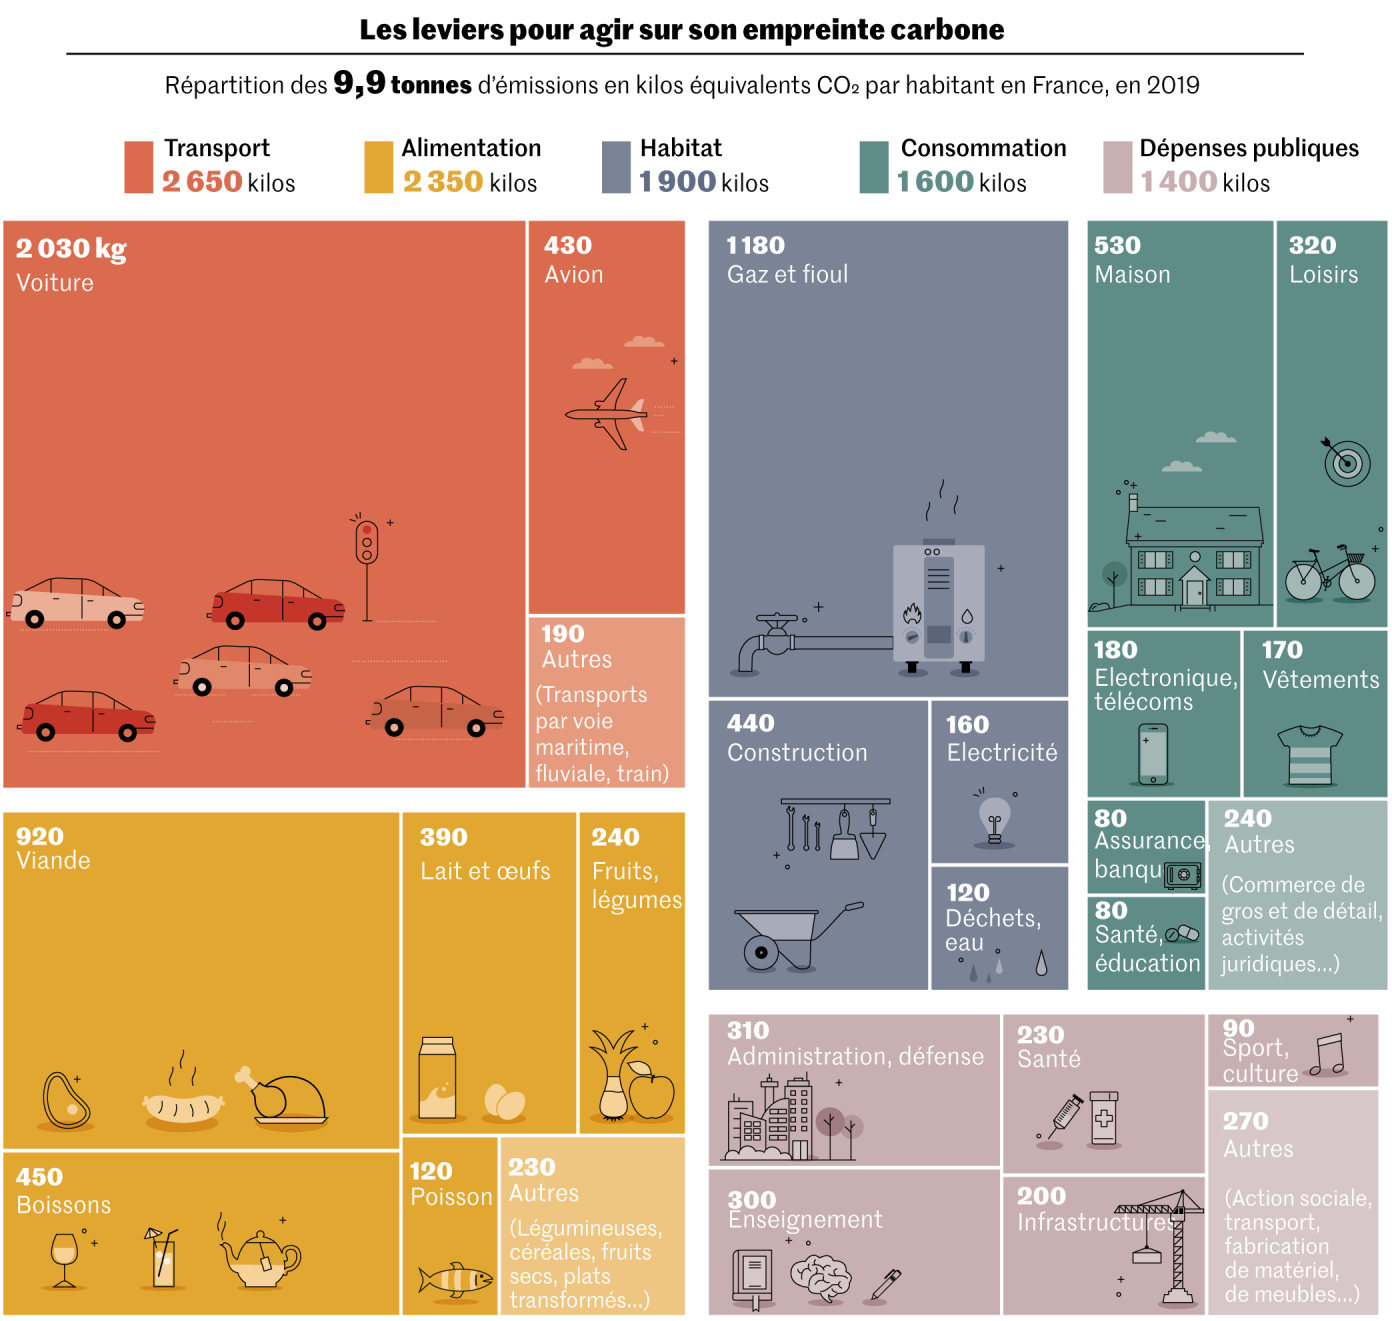
\includegraphics[width=18cm]{carbone}
      
      \ARpartie{Tâche proposée}
         En groupe, trouver une méthode pour vérifier si cette infographie est bien réalisée, en expliquant la méthode. \par
         Récapituler les recherches sur une affiche.
   
   \vfill\hfill {\it\footnotesize Source : d'après une idée de Claire Lommé sur son site \href{https://clairelommeblog.wordpress.com/category/maths-et-societe}{Pierre carrée}.}

\end{Maquette}